\subsection{Pruning without a game}
\label{sec:mechanism}

We start with the simplest possible setting: one informed trader ($I=1$), a
price rule frozen at the monopoly value, no memory, and $\gamma=0$. There is no
rival, no future, and nothing strategic; the optimal order is $v/(2\lambda)$.
Figure~\ref{fig:mechanism} shows the learned intensity relative to the optimum
across 100 independent runs per step size. Standard Q-learning under-trades,
reaching only \MechTakenA{} of the optimal intensity at $\alpha=0.02$ and
\MechTakenE{} at $\alpha=0.4$. The shortfall follows a square-root law,
$1-\hat\beta/\beta^\ast\approx\MechSqrtCoef\sqrt\alpha$ ($R^2=\MechSqrtRsq$).
Counterfactual updating, which credits every order with the profit it would
have earned, learns the optimum at every step size
(\MechCfA--\MechCfE).

The mechanism is the selection effect described in Section~\ref{sec:related}.
With a constant step size, an action's estimate is an exponentially weighted
average of its recent payoffs and fluctuates with standard deviation
proportional to $\sqrt{\alpha}$ times the payoff noise. In a Kyle market the
payoff noise of an order is $\lambda\sigma_u|x|$, so larger orders have noisier
estimates. An order whose estimate dips below the greedy order is updated only
during exploration, so the dip persists; an order whose estimate rises is
chosen and quickly corrected. The asymmetry acts like a penalty proportional
to $\sqrt\alpha\,\lambda\sigma_u|x|$, which shifts the learned order toward
zero by an amount proportional to $\sqrt\alpha$. Counterfactual updates remove
the selection, because every order is updated every period.

This is the over-pruning bias of \citet{dou2025}, here isolated from any
interaction: it alone produces trading intensities 13--57\% below the
optimum. Any test for collusion in a market of such learners must therefore
separate this bias from strategic behaviour.

\begin{figure}[t]
  \centering
  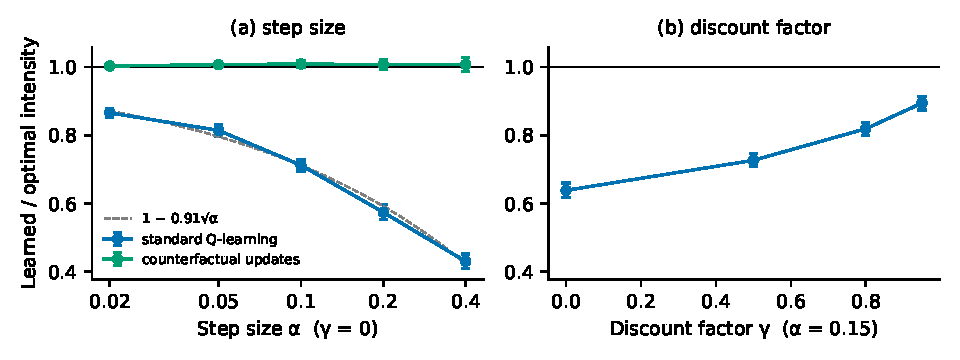
\includegraphics[width=0.5\linewidth]{figures/fig_mechanism.pdf}
  \caption{Pruning without a game. One informed trader facing a fixed price rule
  ($I=1$, $\gamma=0$, no memory, $3\times10^5$ periods, 100 runs per point,
  95\% CIs). Standard Q-learning under-trades by about $0.91\sqrt\alpha$
  (dashed); counterfactual updates learn the optimal order at every step size.}
  \label{fig:mechanism}
\end{figure}
